

\section{Нахождение поля в дальней зоне}

Описанные в разделе~\ref{section:CoreMethod} работы методы численного решения
уравнений Максвелла вместе с описанными в разделе~\ref{section:GridReduction}
методами решения задач на открытых областях дают возможность вычисления
электромагнитного поля внутри некоторой ограниченной области пространства.
Однако на размер этой области накладываются ограничения, вызванные конечной
вычислительной мощностью современных ЭВМ, а~именно тремя основными факторами:
\begin{itemize}
\item ограниченной скоростью выполнения арифметических операций;
\item ограниченным объемом оперативной памяти;
\item ограниченной скоростью обмена данными между процессором
      и оперативной памятью.
\end{itemize}
Поэтому, если нужно рассчитать поле на достаточно большом расстоянии от излучающей
структуры, ресурсов вычислительной техники в случае использования описанного
ранее базового алгоритма может оказаться недостаточно: может не хватить
оперативной памяти или время вычисления окажется неприемлемо большим.

Однако, существует ряд задач, в~которых необходим расчет электромагнитных полей
на~больших расстояниях (в дальней зоне) от~некоторого объекта, излучающего или
рассевающего электромагнитное поле. В~число этих задач входит, например,
получение диаграмм направленности антенн.

Для решения подобных задач существует эффективный способ вычисления полей
в~дальней зоне с~использованием результатов вычисления поля в ближней зоне,
выполненного методом FDTD. Этот способ заключается в~использовании
поверхностного интеграла Кирхгофа.

Интеграл Кирхгофа связывает поле внутри ограниченного объема с~полем и~его
производными на~поверхности, ограничивающей объем. Эта формула была выведена
в~середине XIX~века немецким физиком Гюставом~Кирхгофом, и~во~временной области
имеет следующий вид:
\begin{equation}
    \label{eq:KirchhoffIntegral}
    \Psi(\vect{p},t) = \frac{1}{4\pi} \oint_\Gamma
    \left[
        \frac{1}{R}\nabla'\Psi(\vect{p'},t') -
        \frac{\vect{R}}{R^3}\Psi(\vect{p'},t') -
        \frac{\vect{R}}{cR^2}\frac{\partial}{\partial t'}\Psi(\vect{p'},t')
    \right]_\text{ret} \!\!\!\!\!\vect{n} dA'.
\end{equation}

\noindent
В этом выражении используются обозначения:
\begin{where}
\item $\Psi$ --- любая из шести компонент поля;
\item $\Gamma$ --- поверхность, ограничивающая объем в ближней зоне;
\item $dA'$ --- площадь элемента поверхности;
\item $\vect{n}$ --- единичный вектор нормали к~поверхности;
\item $\vect{p}$ --- точка наблюдения в дальней зоне;
\item $\vect{p'}$ --- точка на~поверхности;
\item $R$ --- расстояние между ними, $\vect{R} = \vect{p}-\vect{p'}$;
\item $c$ --- скорость света в вакууме.
\end{where}

\noindent
В~формуле~\eqref{eq:KirchhoffIntegral} индекс «ret» обозначает тот факт, что
интегрирование осуществляется с~учетом запаздывающего времени~$t'=t-R/c$.
Единичный вектор нормали~$\vect{n}$ всегда направлен внутрь рассматриваемого
замкнутого объема.

Формула~\eqref{eq:KirchhoffIntegral} выражает принцип Гюйгенса, согласно
которому каждая точка на волновом фронте служит фиктивным источником
воображаемой сферической волны. Каждый участок поверхности~$dA'$ излучает волну,
которая приходит в~точку наблюдения с~задержкой~$R/c$. При этом на каждом шаге
FDTD по времени на поверхности интегрирования возникает совокупность фиктивных
источников, поле от которых придет в~точку наблюдения с~разным запаздыванием,
поскольку расстояние~$R$ для всех точек различно. Это означает, что на одном
временном шаге находятся вклад элемента площади~$dA'$ в~разные временные участки
выходного сигнала в~точке наблюдения.

Шаг по времени при вычислении интеграла Кирхгофа тесно связан с~шагом по времени
FDTD и равен ему. Выходная последовательность в~точке наблюдения имеет такой же
шаг по времени. Однако величина~$R/c$ может не быть кратной шагу по времени,
поэтому получаемое время задержки округляется до ближайшего значения, кратного
шагу FDTD. Возникающая при этом ошибка незначительна, т.к. временной шаг
в~классическом FDTD мал по сравнению с~периодом колебаний вычисляемого сигнала.

Выражение~\eqref{eq:KirchhoffIntegral} в~такой форме неудобно для совместного
применения с~методом FDTD. Вывод формул, используемых на~практике, в~данной
работе не приводится и может быть найден, например, в~\cite{bib:Zelenin2006}.
Отметим также, что для получения лучших результатов поверхность интегрирования
следует располагать не в~непосредственной близости от исследуемого объекта, а~на
некотором отдалении от него (порядка 10~шагов дискретизации по~пространству).

Сначала рассмотрим преобразование поля из ближней в дальнюю зону в частотной
области~\cite{bib:Luebbers1991,bib:GodaraHandbook2002}. Окружим
границу TF/SF замкнутой поверхностью~$S$ (см.~рис.~\ref{fig:FarField:SurfaceCurrents}).
Предположим, что~$\vect{n}$ --- нормальный вектор к поверхности~$S$, тогда
определим поверхностные токи на~$S$ как:
\begin{align}
    \vect{J} &=   \vect{n} \times \vect{H}, \\
    \vect{M} &= - \vect{n} \times \vect{E}.
\end{align}
.								(2.23)
В~\cite{bib:Luebbers1991,bib:GodaraHandbook2002} определены векторы
излучения~~$\vect{N}$ и~$\vect{L}$ как:
\begin{align}
    \vect{N} &= \oint\limits_S J e^{jk\vect{r}\vect{r'}} ds, \\
    \vect{L} &= \oint\limits_S M e^{jk\vect{r}\vect{r'}} ds,
\end{align}
%
\begin{where}
\item $\vect{r}$  --- единичный вектор, указывающий на точку наблюдения поля;
\item $\vect{r'}$ --- радиус-вектор точки интегрирования;
\item $k$ --- волновое число;
\item $j$ --- мнимая единица.
\end{where}

Согласно~\cite{bib:Luebbers1991} гармонические составляющие поля в дальней зоне
в полярных координатах могут быть получены из соотношений:
\begin{align}
\label{eq:FarField:LuebbersEquations}
    E_\theta &= - \eta W_\theta - U_\phi, \\
    E_\phi   &= - \eta W_\phi   + U_\theta, \\
    E_r      &=   0, \\
    H_\theta &=   W_\phi - \frac{U_\theta}{\eta}, \\
    H_\phi   &= - W_\theta + \frac{U_\phi}{\eta}, \\
    H_r      &=   0.
\end{align}

Здесь~$\vect{W}$ и~$\vect{U}$ --- векторные величины, заданные следующим
образом:
\begin{align}
    \vect{W} &= \frac{1}{2\lambda R} e^{jkR} \vect{N}, \\
    \vect{U} &= \frac{1}{2\lambda R} e^{jkR} \vect{L}.
\end{align}

\noindent
В этих формулах
\begin{where}
\item $\eta$ --- волновое сопротивление среды;
\item $\lambda$ --- длина волны;
\item $R$ --- расстояние до точки наблюдения поля.
\end{where}

\begin{figure}[p]
\centering
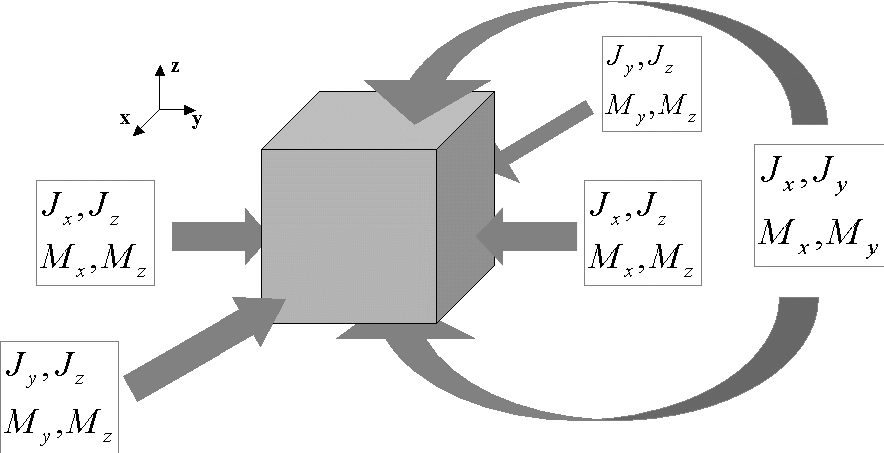
\includegraphics[width=0.7\textwidth]{graphics/far-field-surface-currents}
\caption{Поверхность~$S$ и поверхностные токи.}
\label{fig:FarField:SurfaceCurrents}
\end{figure}

Проведя обратное преобразование Фурье от~\eqref{eq:FarField:LuebbersEquations},
найдем выражения для составляющих поля в дальней зоне во временной области:
\begin{align*}
    E_\theta(t) &= -\eta w_\theta(t) - u_\phi(t), \\
    E_\phi(t)   &= -\eta w_\phi(t) + u_\theta(t), \\
    E_r(t)      &= 0, \\
    H_\theta(t) &= w_\phi(t) - \frac{u_\theta(t)}{\eta}, \\
    H_\phi(t)   &= -w_\theta(t) + \frac{u_\phi(t)}{\eta}, \\
    H_r(t)      &= 0,\\
\intertext{Здесь величины~$w(t)$ и~$u(t)$ расчитываются по следующим формулам:}
    \vect{w}(t) &=
        \frac{1}{4\pi Rc} \frac{\partial}{\partial{t}}
        \oint\vect{j}\left(\textstyle t+\frac{\vect{r}\vect{r'}-R}{c}\right)dS,\\
    \vect{u}(t) &=
        \frac{1}{4\pi Rc} \frac{\partial}{\partial{t}}
        \oint\vect{m}\left(\textstyle t+\frac{\vect{r}\vect{r'}-R}{c}\right)dS.
\end{align*}
Здесь $\vect{j}$, $\vect{m}$ --- поверхностные электрический и магнитный токи
во временной области.
